\chapter{3D case}
\label{chapter:3d}

% {{{1 INTRODUCTION
\section{Introduction}

In this part, we focus on point clouds in 3D that sample a surface. Our goal is
to do the same work as the one done in 2D that is to say smooth the point cloud
using a mean curvature flow approach. This means computing the volume of a union
of balls centered at the points and move the points in the opposite direction to
the one given by the gradient of the volume. An algorithm for computing the
volume can be found in \cite{cazals2011computing}. Since we expect the same
results as in the 2D case (see Chapter \ref{chapter:theory} for a
justification), we preferred to focus to an other kind of flow: an anisotropic
one.

The idea of this flow is to replace the union of balls with a union of convex
polyhedra. The choice of the polyhedron will directly influence the directions
in which the points will be moved.

For doing that, we will replace the Euclidean ball $ B(0, 1) $ with a convex
polyhedron $ B_N(0, 1) $ which can be considered as the unit ball for a certain
norm $ N $. This norm will be called polyhedral (see Section
\ref{sec:polyhedral-norm}). Equation \eqref{eqn:area-union-balls} remains valid if
we replace $ B(p, r) $ with $ B_N(p, r) $ and $ V $ by $ V_N $ (the Voronoi
diagram computed for the norm $ N $) but only if the points are in general
position. Indeed, see Figure \ref{fig:3d-voronoi-cube} for a look at a
particular case where the chosen polyhedron is a cube (norm $ L^\infty $). We
see that if we choose two aligned points, the bisector is not a line and so the
Voronoi diagram does not partition the plane anymore. Furthermore, the
computation of the Voronoi cells for a polyhedral norm is a tough work (see
\cite{ma2000bisectors} for a thorough study). In Appendix
\appendixref{appendix:voronoi-polyhedral-norm}, we study some properties of the
Voronoi diagram for a polyhedral norm and we show that we can symbolically
perturb $ V_N $ in order to get a partition.

\begin{figure}[h]
    \centering

    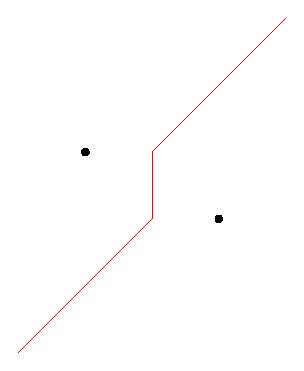
\includegraphics[scale=0.5]{3d/voronoi-cube-non-aligned}
    \hspace{2cm}
    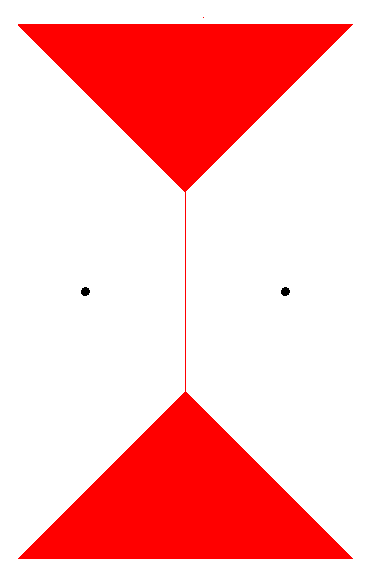
\includegraphics[scale=0.5]{3d/voronoi-cube-aligned}
    \caption{Bisector for the $ L^\infty $ norm: two non aligned points / two
        aligned points}
    \label{fig:3d-voronoi-cube}
\end{figure}

For computing the volume of $ \bigcup_{p \in P} B_N(p, r) $, we implemented two
different methods: a naive one and one based on inclusion-exclusion formula.  In
the naive one, we make the following approximation: instead of summing up over
all intersections $ V_N(p, P) \cap B_N(p, r) $, we sum up over all $ V(p, P)
\cap B_N(p, r) $. The influence of this choice under the functional we minimized
is described in Section \ref{sec:theory-3d-case}. We will see that the second
approached based on inclusion-exclusion formulae is also an approximated one.
There is also one method which is exact but we did not have the time to
implement it in our internship, it is based on 3D arrangements and overlays.

Firstly, we will define formally what we call a polyhedral norm. Then, we will
explain our naive method. Secondly, we will explain the inclusion-exclusion
formula we used in our second method. Then, we will talk about the choices we
made for the implementation and finally, we will run experiments to validate our
expectations.

% {{{1 POLYHEDRAL NORM
\section{Polyhedral norm}
\label{sec:polyhedral-norm}
A polyhedral norm is a function $ N $ defined as follows:

\begin{equation}
    \forall x \in \mathbb{R}^d,~ N(x) = \max_{i} (x | v_i)
\end{equation}
where the $ v_i $ are given vectors from $ \mathbb{R}^d $. This definition
implies that the unit ball for the norm $ N $ is a polyhedron. Indeed, if $ x
\in B_N(0, 1) $, then :

$$ N(x) \leq 1 \Longleftrightarrow \forall i,~(x | v_i) \leq 1 $$

So, the unit ball is defined by linear constraints. More precisely, it is an
intersection of half-spaces and so is a convex polyhedron $ K $. The vectors $
v_i $ are the normal vectors to the facets of $ K $. We will denote by $ B_K(0,
1) $ the unit ball defined by the convex polyhedron $ K $.

% {{{1 VOLUME OF A UNION OF POLYHEDRA
\section{Volume of a union of polyhedra}

In this section, we will show how to compute an approximation of the volume of
a union of polyhedra using two different methods: a naive one and one based on
inclusion-exclusion formula.

% {{{2 NAIVE METHOD
\subsection{Naive method}
We want to compute :

\begin{equation}
    Vol(\bigcup_{p \in P} B_N(p, r)) = \sum_p Vol(\bigcup_p B_N(p, r) \cap V(p, P))
\end{equation}

The idea of this method is to approximate $ Vol(\bigcup_p B_N(p, r) \cap V(p,
P)) $ by $ Vol(B_N(p, r) \cap V(p, P)) $. Then, we just have to compute the
intersection of half-spaces (see Section \ref{sec:3d-implementation} for
details). It is an approximation because, for example, if we want to compute the
perimeter of the boundary of squares in 2D, there is a difference between what
we want to compute and what we actually compute (see Figure
\ref{fig:3d-inclusion-exclusion-squares}): our computation is just an
approximation.

\begin{figure}[h]
    \centering

    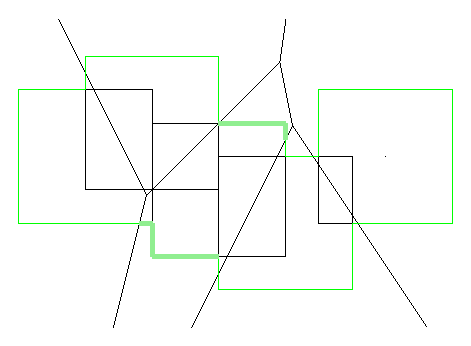
\includegraphics[scale=0.8]{3d/3d_perimeter_squares_truth}
    \hspace{2cm}
    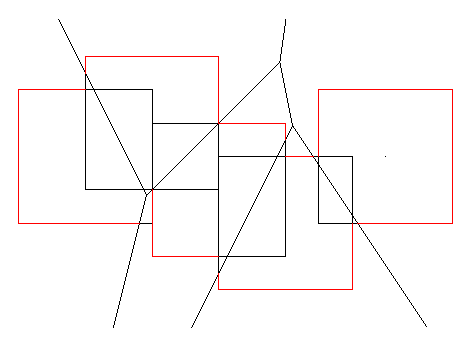
\includegraphics[scale=0.8]{3d/3d_perimeter_squares}
    \caption{In green, what we want and in red what we actually compute}
    \label{fig:3d-inclusion-exclusion-squares}
\end{figure}

% {{{2 INCLUSION-EXCLUSION FORMULA
\subsection{Inclusion-exclusion formula}

The inclusion-exclusion formula is a well-known formula which can be used to
compute the indicator function of a union of sets: given a finite number of sets
$ A = \{ A_1, \ldots, A_N \} $, we have:

\begin{equation}
    \indicator{\bigcup A_i} = \sum_{\emptyset \neq X \subseteq A} (-1)^{card X -
        1} \indicator{\bigcap X}
\end{equation}

This formula can also be expressed using the notion of nerve as shown in
\cite{attali2007inclusion}. We define the nerve of $ A = \{ A_x, x \in X \} $ to
be the simplicial complex \footnote{A simplicial complex is a generalization of
    a triangulation: it is a collection of simplices like vertices, edges,
    triangles, tetrahedra...} where a simplex $ \sigma $ exists between $ x_1
\ldots, x_k $ if $ \bigcap\limits_{i=1}^k A_{x_i} \neq \emptyset $. Then, we can
write the inclusion-exclusion formula as:

$$ \indicator{\bigcup A_x} = \sum_{\sigma \in Nerve(A)} (-1)^{\dim \sigma}
\indicator{\bigcap \sigma} $$
$ \sigma $ represents any simplex in the nerve. Its dimension is defined as: $
\dim \sigma = card \sigma - 1 $. If we consider a union of polyhedra, we can write a similar formula:

\begin{equation}
    \indicator{\bigcup B_N(p, r)} = \sum_{\sigma \in Nerve(\mathcal{B}_N)} (-1)^{\dim \sigma}
    \indicator{\bigcap \sigma}
    \label{eqn:incl_excl_simplices}
\end{equation}
where $ \mathcal{B}_N $ is the collection of all balls $ B_N(p, r), p \in P $.

Now, since the nerve can be a really big object, we want to restrict the
computation to what we call the $\alpha$-complex of a set of points:

\begin{definition} The $\alpha$-complex of a set of points $ X $ denoted by $
    Del(X, \alpha) $ is a subset of the Delaunay triangulation. To each simplex
    of the Delaunay triangulation, we can associate a characteristic
    radius: the radius of the smallest empty circle containing the simplex.

    Now, the $\alpha$-complex contains all the simplices of the Delaunay
    triangulation whose characteristic radius is smaller than $\alpha$.
\end{definition}

Now, we can ask if the formula \ref{eqn:incl_excl_simplices} is still valid if
we replace $ Nerve(\mathcal{B}_N) $ by $ Del(P, r) $.

If we want to prove this assertion, we may use the technique used to prove the
inclusion-exclusion formula for a union of balls. The proof starts by defining
the subcomplex $ L_p $ induced by a vertex $ p $.  We consider all the
polyhedrons that contains a given point $ x $ and we construct the nerve of it.
Formally, $ L_x = Nerve(\{ B_N(p, r),~x \in B_N(p, r)\}) $.

Then, when we evaluate the indicator function at $ x $ of the union, we can
decompose it in two parts: simplices of $ L_x $ and the other ones.

\begin{align*}
    \indicator{\bigcup B_N(p, r)}(x) &= \sum_{\sigma \in L_x} (-1)^{\dim \sigma}
    \indicator{\bigcap \sigma}(x) + \sum_{\sigma \notin L_x} (-1)^{\dim \sigma}
    \underbrace{\indicator{\bigcap \sigma}(x)}_{= 0 \text{ since } x \notin
        \sigma} \\
    &= \sum_{\sigma \in L_x} (-1)^{\dim \sigma} \\
    &= \chi(L_x)
\end{align*}

Here, $ \chi $ is the Euler characteristic.

Now, if we show that $ L_x $ is contractible (can be continuously deformed to a
point), we know that $ \chi(L_x) = 1 $. Obviously, we also have $
\indicator{\bigcup B_N(p, r)}(x) = 0 $ if $ x $ is not in the union and we will
conclude that the formula \ref{eqn:incl_excl_simplices} is true. But it appears
that there exists cases where the formula is not correct: see Figure
\ref{fig:incl_excl-examples}. In this figure, we can see that in the
$\alpha$-complex for the $ L^\infty $ norm, the triangle does not exist. It
means that in the formula the intersection between the three squares will not be
taken into account and so the final result will be incorrect. During this
internship, we did not have the time to estimate the error made by using this
formula.

\begin{figure}[h]
    \centering
    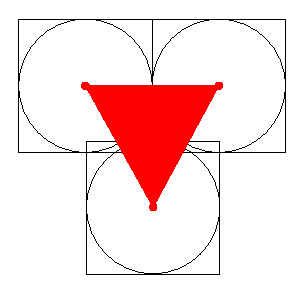
\includegraphics[scale=0.7]{3d/inclusion-exclusion-counter-l2}
    \hspace{2cm}
    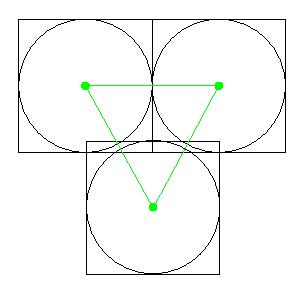
\includegraphics[scale=0.7]{3d/inclusion-exclusion-counter-linfty}
    \caption{Counter example where the formula is not correct, in red the
        $ L^2$ $\alpha$-complex and in green the $ L^\infty$ $\alpha$-complex.}
    \label{fig:incl_excl-examples}
\end{figure}

% {{{1 IMPLEMENTATION DETAILS
\section{Implementation details}
\label{sec:3d-implementation}

In this section, we will describe briefly how we implemented the two methods
previously described.

% {{{2
\paragraph{Intersection computation}

For both methods, we need a way to compute an intersection of half-spaces: for
the first one, we need to compute the intersection of a Voronoi cell and a
convex polyhedron and for the second one, we need to compute intersections of
convex polyhedra.

For the first method, the naive one, a Voronoi cell is represented implicitly as
a list of half-spaces (the planes defining the boundary of the cell).
Half-spaces are computed using the Delaunay triangulation. If we want to compute
the Voronoi cell of $ p $, we look at the neighbours of $ p $ in the Delaunay
triangulation. Then, for every neighbour $ v $, the corresponding half-space is
the positive part of the bisector plane between $ p $ and $ v $. The latter is
the  plane passing through the midpoint of the segment $ [p, v] $ and whose
normal vector is $ \vec{pv} $. Since the traversal order of the vertices of the
Delaunay triangulation is not, in general, the same as the insertion one, we
need to associate an index to each point (using a simple \texttt{std::map}).

Recall that a convex polyhedron $ K $ represents the unit ball for a polyhedral
norm $ N $. $ K $ is internally represented as a list of normal vectors to each
of its facets. Using this representation, one can compute the translated
polyhedron $ B_N(p, r) $ for a point $ p $ and a radius $ r $ by noticing that
it is the intersection of the half-spaces $ H_n $ where $ H_n $ is defined, for
any normal vector $ n $, as follows: $ H_n = \{ x \in \R^3,~ (x | n) \leq (p |
n) + r \} $

In order to construct this intersection, we used the duality which allows us to
replace the computation of an intersection by the computation of a convex hull
(see \cite{preparata1979finding}) of dual points. The duality is defined as
follows: for any halfspace defined as the positive part of a plane $ p $ which
does not contain the origin and whose Cartesian equation is $ ax + by + xz + d =
0 $, the corresponding dual point is given by $ (-\frac{a}{d}, -\frac{b}{d},
-\frac{c}{d}) $.

Concretely, we compute the intersection in the following manner (see
\appendixref{appendix:code-intersection} for a simplified version of the
algorithm):
\begin{enumerate}
    \item Compute the dual points while remembering which point is associated to
        which plane.
    \item Compute the convex hull of these dual points. It gives us a dual
        polyhedron. To each vertex of this polyhedron, we associate the
        corresponding primal plane.
    \item To compute the primal polyhedron:
        \begin{enumerate}
            \item We first compute the primal vertices which are the dual of the
                dual facets: each dual facet has at least 3 vertices. We know
                the corresponding primal planes for these vertices.  Then, the
                corresponding primal vertex is the intersection of the 3 primal
                planes.
            \item Secondly, primal facets are constructed by circulating
                around the dual vertices. Each time there is an edge between two
                dual vertices, there is an edge between the two corresponding
                primal vertices.
        \end{enumerate}
\end{enumerate}

For the second method, we also need a way to compute the $\alpha$-complex of a
set of points. This can be done using the \texttt{Alpha\_shapes\_3} package of
\texttt{CGAL} and the associated classification methods.

% {{{2
\paragraph{Automatic Differentiation integration}

Let us now explain in more details the integration of the automatic
differentiation tool. \texttt{CGAL} has the particularity to make things easy
for the programmer to change the number type by using the concept of a
\emph{Kernel}. A \emph{Kernel} is a class that describes how numbers are stored
in memory, how we can construct things (like points, planes, bisectors...) and
how to evaluate predicates on objects (collinearity test, coplanarity test...).

There are multiple predefined kernels but we will quickly talk about two
particular ones. \texttt{Simple\_cartesian<NT>} is the most basic one: a number
will just be represented by \texttt{NT} and so it has inexact predicates
evaluation and inexact constructions since it is subject to numerical errors.

\texttt{Exact\_predicates\_inexact\_constructions\_kernel} (in short
\texttt{Epick}) is a Kernel which uses a technique called \emph{filtering} to
ensure that the predicates are always evaluated in an exact manner. In short,
the predicate is first evaluated in an inexact way using interval arithmetic.
If the predicate, for example, has to check whether a value is zero or not then,
using interval arithmetic, it will need to check whether the resulting interval
contains zero or not. If this interval does not contains zero, then a decision
can be made. Otherwise, the computation is done again but this time using exact
arithmetic which, in all cases, will return an answer.

For the automatic differentiation, we replaced the \texttt{NT} type with a
custom class \texttt{AD}. \texttt{AD} is a class with two members: a value and a
vector of derivatives. It overloads all the classical arithmetic operators such
as addition, subtraction, multiplication, division. It also overloads, using the
chain rule, some mathematical functions such as \texttt{sqrt}, \texttt{atan2}...
For example, the implementation of \texttt{sqrt} for AD looks like this:
\lstinputlisting[language=C++]{code/sqrt_AD.h}

Then, for interfacing \texttt{AD} with \texttt{CGAL}, we choose the
\texttt{Simple\_cartesian<AD>} kernel. The choice of \texttt{Simple\_cartesian}
may seem inappropriate at first glance because the constructions are inexact but
it is enough for our applications. In practice, we use a combination of
\texttt{Epick} and \texttt{Simple\_cartesian<AD>}. For example, when computing
an intersection of half-spaces, we construct the dual using \texttt{Epick} to
have the exact combinatorics of the dual. Then, we use
\texttt{Simple\_cartesian<AD>} when we effectively construct the primal
polyhedron.

% {{{1 EXPERIMENTS
\section{Experiments}

% TODO

We compare the two different methods using various polyhedra and point clouds.
If we choose a polyhedron sufficiently close from the unit sphere, we expect the
result to be the same as in the 2D case: gradients should be oriented like the
outward normal with a norm proportional to the mean curvature.

Figure \ref{fig:3d-mean-curvature-sphere-cube} gives an example where the point
cloud is a sphere and the polyhedron is a cube.

\begin{figure}[h]
    \centering
    \begin{minipage}{0.32\linewidth}
        \centering
        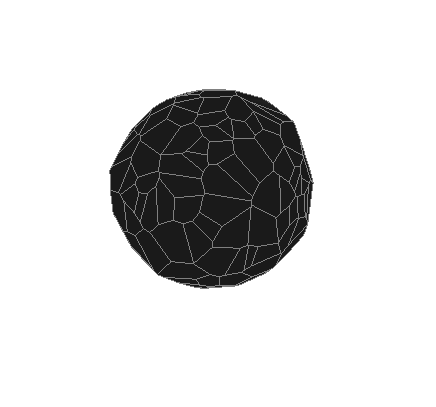
\includegraphics[scale=0.35]{3d/sphere-polyhedron-200}
        \subcaption{Discretized sphere with 200 planes}
    \end{minipage}
    \begin{minipage}{0.32\linewidth}
        \centering
        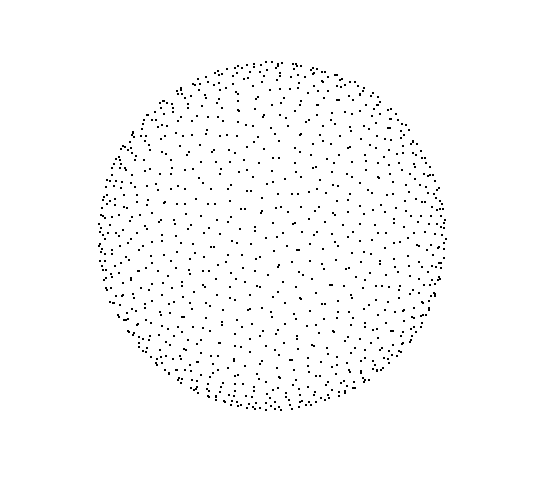
\includegraphics[scale=0.3]{3d/sphere-1000}
        \subcaption{Initial point cloud: 1000 points on a sphere}
    \end{minipage}
    \begin{minipage}{0.32\linewidth}
        \centering
        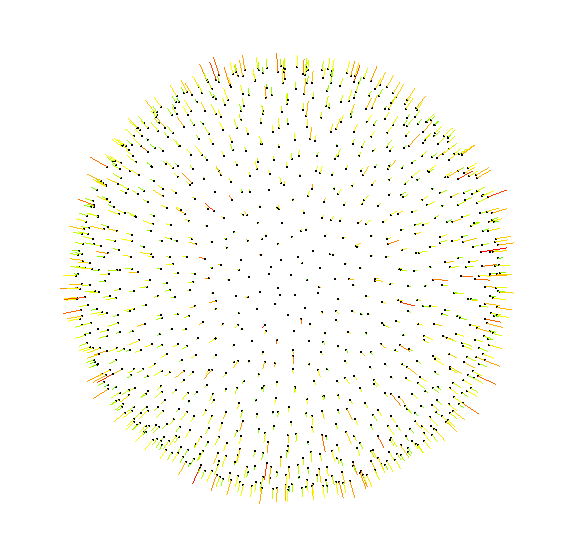
\includegraphics[scale=0.3]{3d/sphere-sphere-1000-05}
        \subcaption{Gradients of the volume}
    \end{minipage}
    \caption{Sphere / cube}
    \label{fig:3d-mean-curvature-sphere-cube}
\end{figure}

We observe that the gradients are oriented like the outward normals and that
norms of these gradients seem relatively constant. This confirms the fact that
we can simulate our work in 2D (mean curvature flow) by choosing a sufficiently
discretized sphere.

We also did some experiments for checking the convergence of the flow. Figures
\ref{fig:3d-flow-sphere-cube} and \ref{fig:3d-flow-sphere-bipyramid} give
examples where the point cloud is a sphere and the polyhedron is a cube and a
bipyramid. On these examples, we can see that the flow seems to converge towards
the polyhedron we choose.

\begin{figure}[h]
    \centering
    \begin{minipage}{0.32\linewidth}
        \centering
        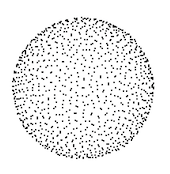
\includegraphics[scale=0.4]{3d/sphere-cube-0}
        \subcaption{Initial sphere with 1000 points}
    \end{minipage}
    \begin{minipage}{0.32\linewidth}
        \centering
        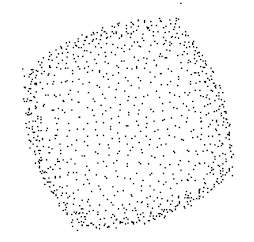
\includegraphics[scale=0.4]{3d/sphere-cube-10}
        \subcaption{After 10 iterations}
    \end{minipage}
    \begin{minipage}{0.32\linewidth}
        \centering
        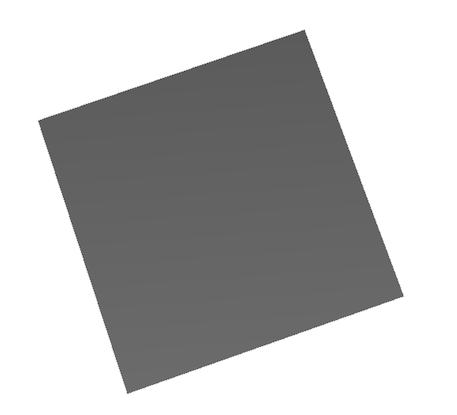
\includegraphics[scale=0.3]{3d/sphere-cube-cube}
        \subcaption{Shape of the cube}
    \end{minipage}

    \caption{Flow of a sphere under a cube}
    \label{fig:3d-flow-sphere-cube}
\end{figure}

\begin{figure}[h]
    \centering
    \begin{minipage}{0.32\linewidth}
        \centering
        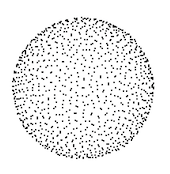
\includegraphics[scale=0.4]{3d/sphere-cube-0}
        \subcaption{Initial sphere with 1000 points}
    \end{minipage}
    \begin{minipage}{0.32\linewidth}
        \centering
        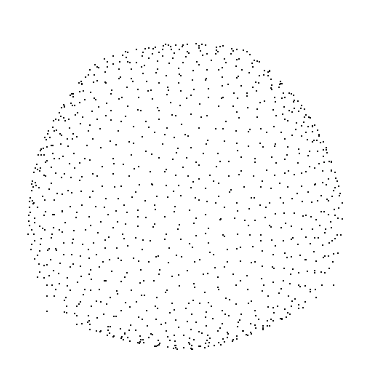
\includegraphics[scale=0.4]{3d/sphere-bipyramid-10}
        \subcaption{After 10 iterations}
    \end{minipage}
    \begin{minipage}{0.32\linewidth}
        \centering
        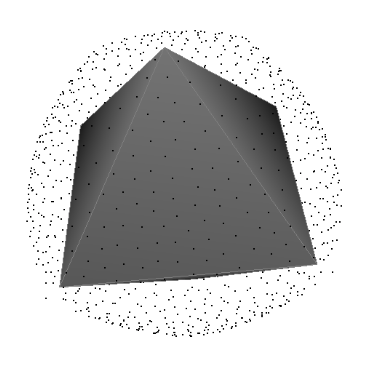
\includegraphics[scale=0.3]{3d/sphere-bipyramid-bipyramid}
        \subcaption{Shape of the bipyramid}
    \end{minipage}

    \caption{Flow of a sphere under a bipyramid}
    \label{fig:3d-flow-sphere-bipyramid}
\end{figure}

% {{{1 CONCLUSION
\section{Conclusion}

In summary, we saw, in this chapter, another type of flow. We used the same
techniques as the ones developed in Chapter \ref{chapter:2d} by replacing a
union of balls with a union of convex polyhedra.

We saw that the obtained flow has different properties than the mean curvature
flow: the convergence shape will depend on which polyhedron we chose.

% TODO:

% TODO:
% - comparaison des différentes méthodes
% - résultats

% vim: set spelllang=en filetype=tex :
